\chapter{Evaluation}
\label{chapter:evaluation}

\section{Tests Objectives}

The test conducted were chosen in order to evaluate the fulfillment of this thesis goals.

Our system leverages user detection to improve occupant comfort and reduce wasted energy and because of that we require the user detection to be achieved in a reasonable time frame.

The motion detection feature of our system is important to achieve room security and monitoring, for that reason we need to ensure the system has a good success rate. 

The temperature and luminosity sensors have an important role in ensuring our system has the correct information to perform building automation and increase user comfort, by adjusting the temperature and lights. 

Another objective is to test the Hub web-server ability to respond to a few concurrent users. Since the server is intended to serve a single office room we don't expect tens of concurrent user.

Finally we need to determine if users fell comfortable using our system. If they experienced any problems with the \ac{UI}, those problems need to be corrected.


\section{Tests Scenarios}



All the tests were conducted in real scenarios inside an office of the \ac{IST} - Taguspark campus. They
were executed using the hardware described in Section~\ref{hardware_arch_imp}, and one Moto G3 phone running the user app.


\subsection{User detection - Room}


In order to test the  user detection time in the office, a series of measurements were performed. The test consists in observing the time the user app takes to detect the Estimote beacon present inside the office (beacon with 3.5 meter range). The user will start walking from just outside the beacon range and walk normally to the office door.

The measurements were performed with the beacon device in the center of office. The user's phone was a Moto G3 Android phone with BT support up to version 4.0 .
For testing purposes, the user app was set to vibrate when it was near the beacon in order for us to know if it found the beacon. A chronometer was be used to determine the reaction time. The test resulted in 20 measurements that were used to determine a meaningful average of the reaction time of the system.


\subsection{User detection - Building}

In order to test the reaction time of user detection in the building, a series of measurements were performed. The test consists in observing the time the user app takes to detect the phone is inside the building. The user will start walking from the front door of the building to the office door.

The device used was a Moto G3 Android phone with WiFi 802.11 b/g/n support.
For testing purposes the user app is set to vibrate when it is inside the building. A chronometer will be used to determine the reaction time. The test resulted in 20 measurements that were used to determine a meaningful average of the reaction time of the system.



\subsection{Motion detection}

To test the motion detection, a series of measurements were performed to test the algorithm. The test consists in a person walking in front of the Hub camera at different speeds from the door to a desk. This test will show if our system is able to detect motion when people enter the office and if it can be tricked into producing false negatives results.




\subsection{Temperature and Luminosity}

This test measures the correct behavior of the built-in luminosity sensor and the external temperature sensor (Arduino based). 

The luminosity test consists in reading the sensor data in a room with no lights on, and then turn on the lights to determine if a change in the sensor was observed.

To test the Arduino based temperature sensor the \ac{HVAC} system will be turned on, and the temperature readings will show if changes in temperature in the office were observed.


\subsection{Hub server load}


To test our system's web-server a series of measures were performed. This test consists of making several concurrent \ac{HTTP} requests to the server in the Hub app. To send these requests we used the \ac{ab}\footnote{http://httpd.apache.org/docs/2.4/programs/ab.html} benchmarking tool.

The goal of this test is to determine if the server handles a small amount of concurrent users. The website is not expected to server hundreds of concurrent users, instead it will handle a few users sending occasional POST requests and some periodic GET requests to keep the user app updated when in use.


\subsection{Automation}

To evaluate the usability of the \ac{IFTTT} interface (automation recipes), user usability tests were performed with a total of 20 users. The users who performed the tests were not familiar with our system and had no previous experience with similar \ac{IFTTT} solutions.

The users were asked to create two distinct recipes:

\begin{itemize}
  \item If the user left the office, then turn off all the lights.
  \item If the temperature is above 25 ºC, then set temperature to below 20 ºC. 
\end{itemize} 

The test results were then compared to an expert user to determine the usability of the system.



\section{Test Results}


\subsection{User detection - Room}

A set of measurements were taken in order to determine the response time the application takes to identify the user's phone is inside the room. Two types of measurements were taken.

In the first test, the user is inside the room with \ac{BT} turned off, then it was turned on and the timer started, Figure~\ref{eval:room} shows the cumulative distribution function obtained from the measurements. 

In the second set of measurements, the user starts walking outside the office and the timer starts when he opens the unlocked door to the room. The cumulative distribution function for the second test is shown in Figure~\ref{eval:room2}.

In the first test we observed that in most cases our system detected the user presence very quickly within a few seconds but in other occasions, it seemed to take up to 22 seconds. We noticed once it detected the Estimote beacon the first time it found it correctly the following times, but seems to take some time for the initial discovery. Looking at the second test, where the user enters the room, we see worse results in comparison to the first test. The maximum time increased to 27 seconds. We consider the time to detect the user presence is adequate for turning on the \ac{HVAC} system in the user presence, but not perfect for turning on the lights when the user enters the room.

For cases when the user wants the lights to be on when he enters the room and if the detection time is considered insufficient, a automation recipe can be created for turning on the light when movement is detected and the user is inside the building. Nevertheless, we consider the room detection time adequate for rooms with ambient light from a window but not for dark rooms.

The office where the tests were conducted is roughly 3 by 6 meters wide. The Estimote beacon range was set to approximately 3.5 meters. Regarding false positives, the beacon signal can be observed in the adjacent office when next to the wall between the rooms. This means our system can incorrectly identify the user presence when inside an adjacent office next to the wall. A possible solution to this problem is to use more than one beacon with range set to 1.5 meters and spread them in the room. Since the range is shorter the signal won't be so easily detected in adjacent rooms but still offers coverage of the target room.


\begin{figure}[]
\centering
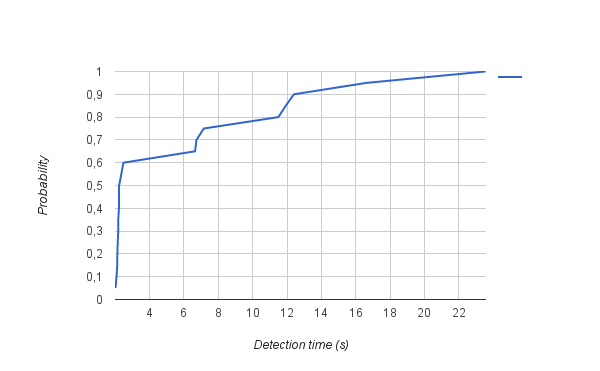
\includegraphics[width=0.9\textwidth]{Figures/room_detection_cumulative}
\caption{Cumulative distribution function of the time it takes to detect a user inside a room}
\label{eval:room}
\end{figure}

\begin{figure}[]
\centering
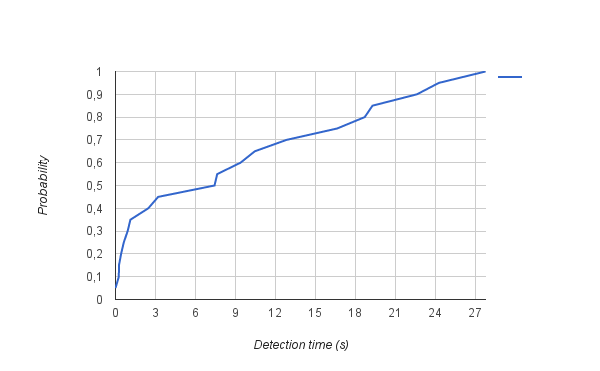
\includegraphics[width=0.9\textwidth]{Figures/room_detection_cumulative2}
\caption{Cumulative distribution function of the time it takes to detect a user when he enters the room}
\label{eval:room2}
\end{figure}

%\begin{table}[]
%\centering
%\begin{tabular}{|r|r|}
%\hline
%\multicolumn{1}{|c|}{Test 1} & \multicolumn{1}{c|}{Test 2} \\
%\multicolumn{1}{|l|}{\begin{tabular}[c]{@{}l@{}}Time (seconds) to detect user \\ presence in room, when user \\ is already inside\end{tabular}} & \multicolumn{1}{l|}{\begin{tabular}[c]{@{}l@{}}Time (seconds) to detect user \\ presence in room, when user \\ is outside and walks inside\end{tabular}} \\ \hline
%2.13 & 7.63 \\ \hline
%2.23 & 3.20 \\ \hline
%2.02 & 18.70 \\ \hline
%23.55 & 27.76 \\ \hline
%6.65 & 24.26 \\ \hline
%11.5 & 2.46 \\ \hline
%7.16 & 0.91 \\ \hline
%2.36 & 0.42 \\ \hline
%2.18 & 22.62 \\ \hline
%2.48 & 0.62 \\ \hline
%12.4 & 1.12 \\ \hline
%2.15 & 10.45 \\ \hline
%6.73 & 16.63 \\ \hline
%2.18 & 0 \\ \hline
%11.93 & 0.26 \\ \hline
%2.22 & 0.25 \\ \hline
%2.12 & 19.28 \\ \hline
%16.62 & 7.43 \\ \hline
%2.08 & 12.83 \\ \hline
%2.23 & 9.38 \\ \hline
%\end{tabular}
%\caption{Room detection measurements}
%\label{eval:room}
%\end{table}
%
%
%\begin{table}[]
%\centering
%\begin{tabular}{l|r|r|}
%\cline{2-3}
% & \multicolumn{1}{l|}{Test 1 (s)} & \multicolumn{1}{l|}{Test 2 (s)} \\ \hline
%\multicolumn{1}{|l|}{Mean} & 6.14 & 9.31 \\ \hline
%\multicolumn{1}{|l|}{Standard deviation} & 5.92 & 9.03 \\ \hline
%\end{tabular}
%\caption{Room detection  - Mean and Standard deviation for tests when the user is inside and walks inside the room}
%\label{eval:room2}
%\end{table}





\subsection{User detection - Building}

Several measurements were taken to determine the time the application takes to detect that the user is inside the building. The cumulative distribution function from the measurements is shown in Figure~\ref{eval:building1}.

Building level user detection does not need very quick response times, unlike room detection, as building location will be mostly used to preheat the room before the user arrives. The response time observed shows an acceptable response time.



Our building \ac{WiFi} range extends a few meters beyond the front door so in some measurements our system detected the user before he walked through the front door of the building.

\begin{figure}[]
\centering
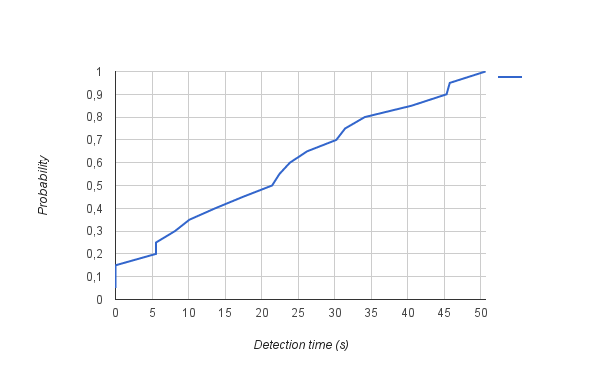
\includegraphics[width=0.9\textwidth]{Figures/building_detection_cumulative}
\caption{Cumulative distribution function of the time it takes to detect a user  after he enters the building}
\label{eval:building1}
\end{figure}





%\begin{table}[]
%\centering
%\begin{tabular}{|l|}
%\hline
%Time (seconds) \\ \hline
%21.44 \\ \hline
%40.54 \\ \hline
%0 \\ \hline
%5.55 \\ \hline
%30.23 \\ \hline
%10.12 \\ \hline
%0 \\ \hline
%5.54 \\ \hline
%34.12 \\ \hline
%8.14 \\ \hline
%0 \\ \hline
%22.43 \\ \hline
%45.32 \\ \hline
%50.65 \\ \hline
%26.24 \\ \hline
%31.43 \\ \hline
%45.76 \\ \hline
%13.65 \\ \hline
%17.43 \\ \hline
%23.87 \\ \hline
%\end{tabular}
%\caption{User building detection, the time to detect the user starting in the building front door}
%\label{eval:building1}
%\end{table}



\subsection{Motion detection}

To test motion detection, we conducted tests with three different people with different heights. Each person entered the room at different speeds, the obtained results are shown in Table~\ref{eval:motion}.

Our system was able to correctly identify a person walking inside the room every time. Figure~\ref{eval:motion_fig} shows an example of the different pixels in the camera frames identified by our algorithm. Regarding false positives, from object motion they don't seem to be a big problem since our system allows the creation of a no-monitoring-area in the camera frame to use in cases of rooms with window view.

The motion test was performed during day hours, in these conditions the camera is able to capture good frames. We did not perform test during the night time  but likely our system will have problems detecting movement in completely dark rooms. To fix this problem we can install sensors to detect if the office door is open. If the door is opened and there is not enough light our system could turn on the lights momentarily to enable motion detection.


\begin{table}[]
\centering
\begin{tabular}{|l|l|l|l|}
\hline
 & \begin{tabular}[c]{@{}l@{}}Person 1\\ detection\end{tabular} & \begin{tabular}[c]{@{}l@{}}Person 2\\ detection\end{tabular} & \begin{tabular}[c]{@{}l@{}}Person 3\\ detection\end{tabular} \\ \hline
Slow walk & 20/20 & 20/20 & 20/20 \\ \hline
Normal walk & 20/20 & 20/20 & 20/20 \\ \hline
Run & 20/20 & 20/20 & 20/20 \\ \hline
\end{tabular}
\caption{Motion detection tests for three people with different heights, 20 measurements each.}
\label{eval:motion}
\end{table}


\begin{figure}[]
\centering
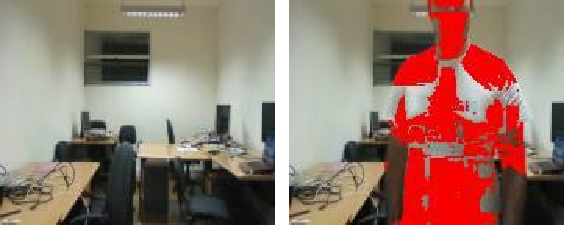
\includegraphics[width=0.7\textwidth]{Figures/eval_motion}
\caption{Motion detection - Frame before and after, motion detected }
\label{eval:motion_fig}
\end{figure}



\subsection{Temperature and Luminosity}

In order to test the functionality of the luminosity and temperature sensors in the system, these were used to collect ambient data.

To test the luminosity sensor behavior we turned on the lights in the room and allowed the Hub to record the values for a while, then we turned off the lights and waited for a few minutes then repeated the same steps one more time. In Figure~\ref{eval:lights} we can observe two different gaps where the lights were off. As expected the Android luminosity sensor operates as intended and provides the system with correct data. During the first test period of no lights a computer monitor was turned on and that caused the luminosity values to be a bit above zero.

To test the external temperature sensor, the HVAC system was turned on and the temperature was recorded. In Figure~\ref{eval:temp} we can observe a small decline in the temperature after the HVAC system was turned on. The temperature was lowered by 2ºC and then went back to the 24 ºC after the HVAC system was turned off.

\begin{figure}[]
\centering
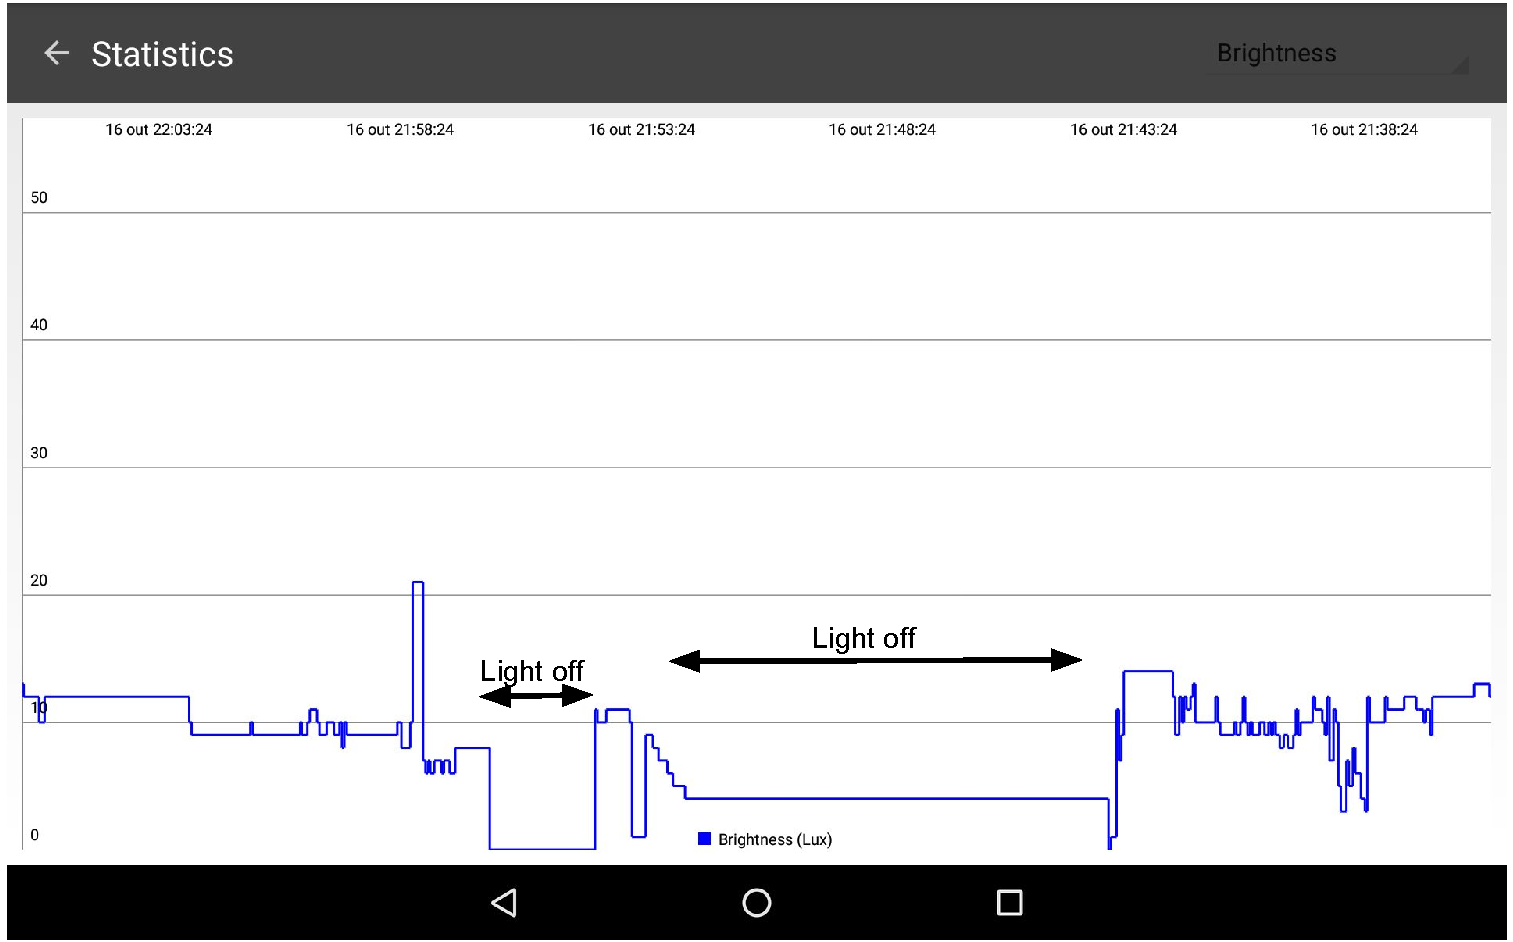
\includegraphics[width=0.8\textwidth]{Figures/eval_lights}
\caption{Luminosity Readings}
\label{eval:lights}
\end{figure}

\begin{figure}[]
\centering
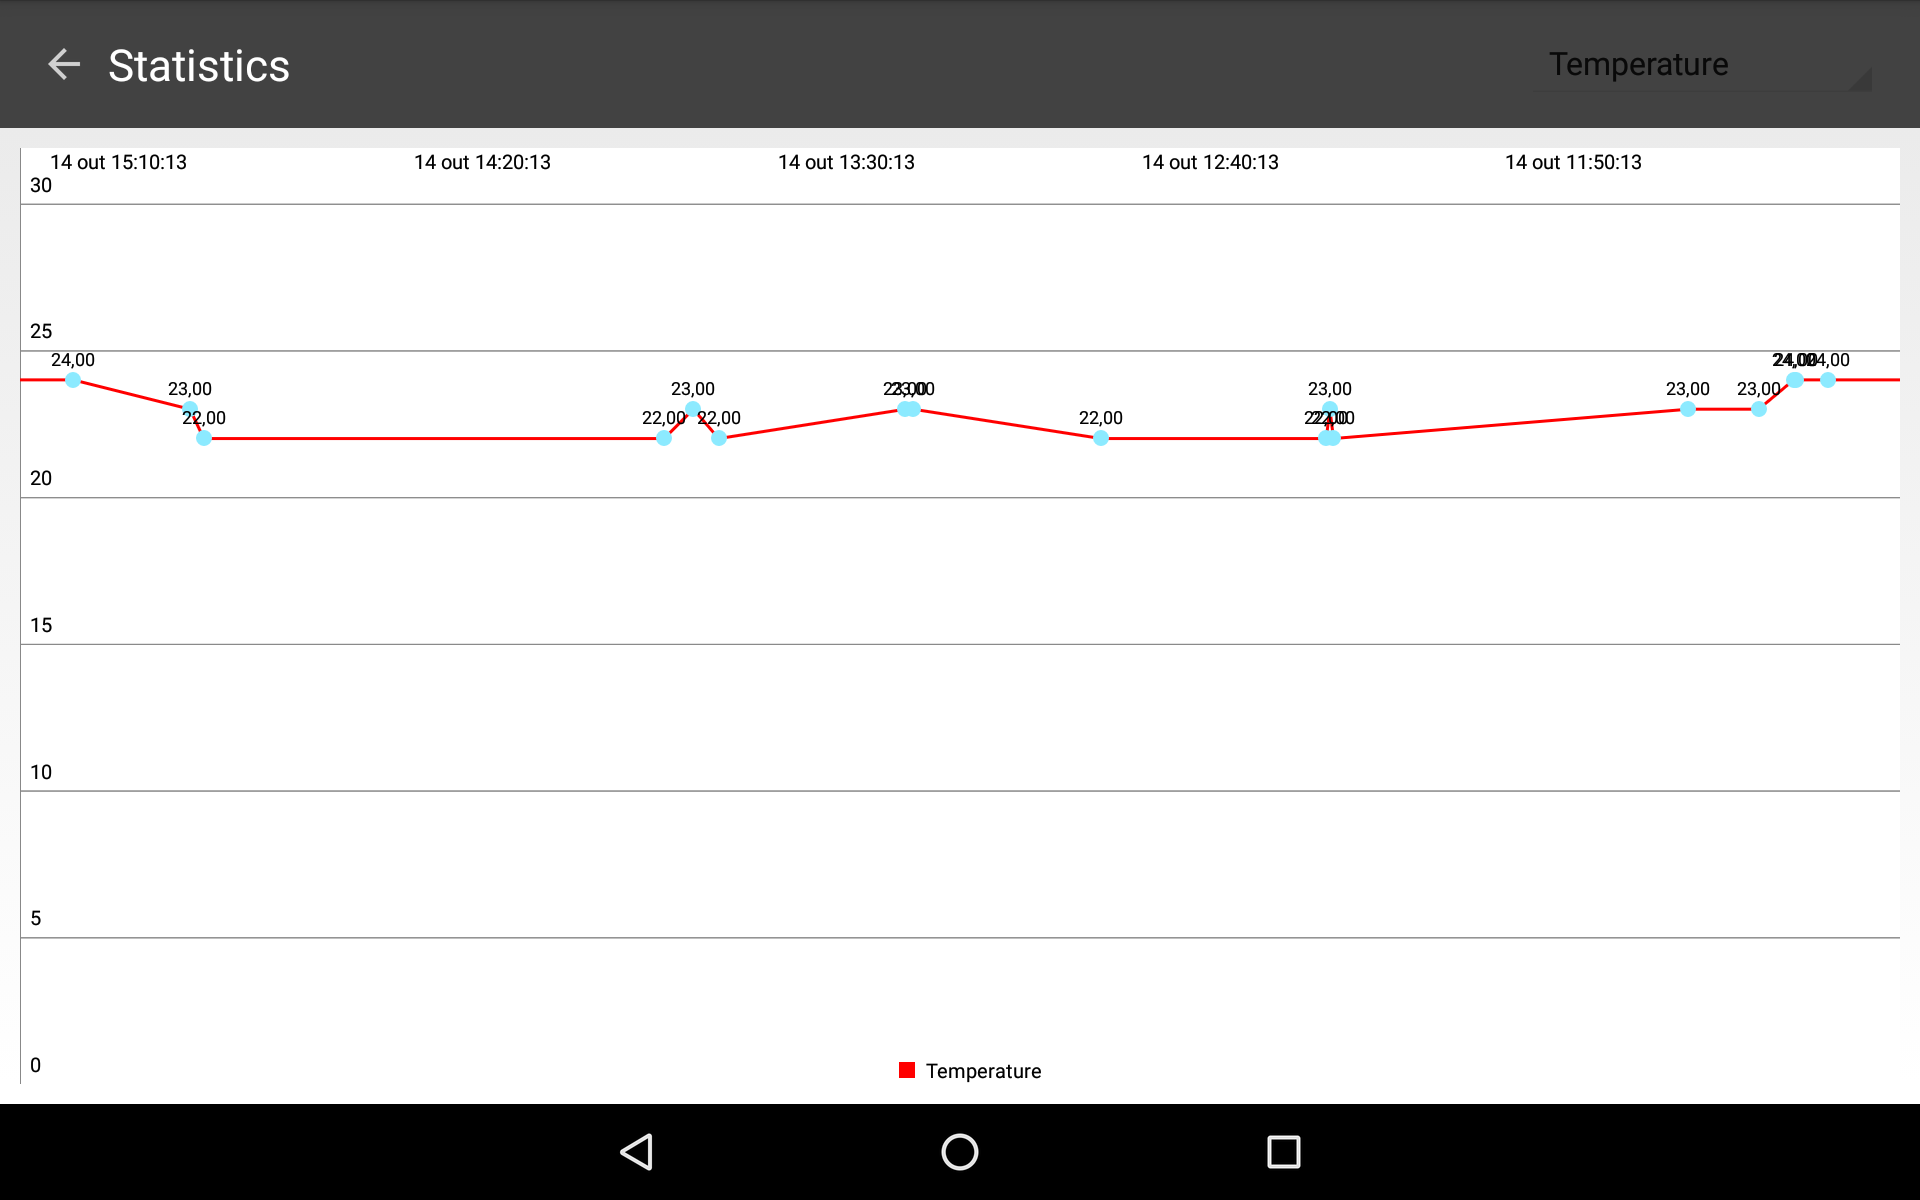
\includegraphics[width=0.8\textwidth]{Figures/eval_temp}
\caption{Temperature Readings}
\label{eval:temp}
\end{figure}


\subsection{Hub server load}

To test the web server, we used \ac{ab} to send requests during 5 minutes with different concurrency levels. This simulates multiple users sending concurrent requests to our server.

Two scenarios were tested:
\begin{itemize}
  \item Users sending GET request to /status endpoint to retrieve the current temperature and light state .
  \item Users sending POST request to /make-changes endpoint to change the temperature and the lights.
\end{itemize} 

Both scenarios were repeated for different concurrency levels (1, 10, 50, 100, 150, 200). For each concurrency levels the test was repeated 5 times in order to obtain an average value. 

The results of this test are shown in Figures~\ref{eval:server1} and \ref{eval:server2}. We determined our website is able to respond within 500 ms with 100 concurrent users and no errors. We believe this value is more than adequate for the expected load the server will handle for normal office rooms with few people. Even if this system is used in a large room with a few dozens of people it would still perform it's job.


The results obtained in this test used a specific Android tablet with 2GB of Ram and quad-core CPU a 2013 Nexus 7. Different Android devices may present different results from the ones observed in these tests. 

\begin{figure}[H]
\centering
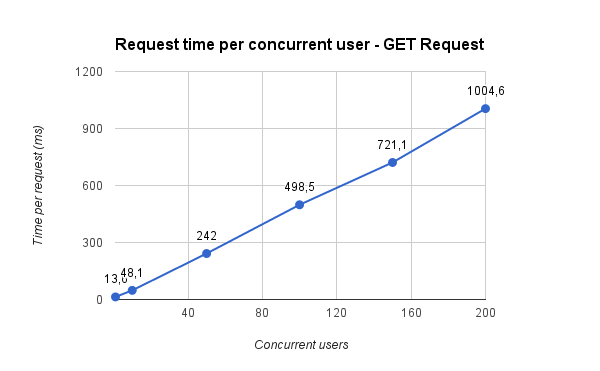
\includegraphics[width=0.7\textwidth]{Figures/bench_get}
\caption{Get Request time per concurrent user.}
\label{eval:server1}
\end{figure}

\begin{figure}[H]
\centering
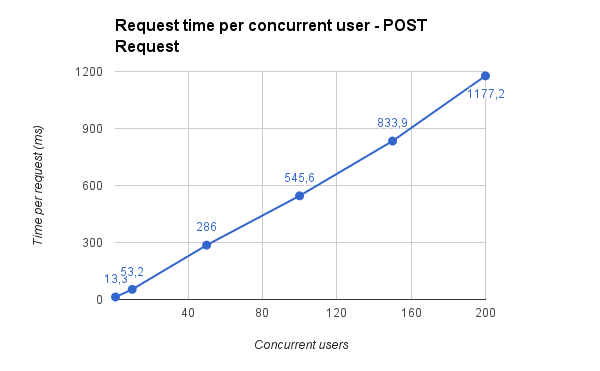
\includegraphics[width=0.7\textwidth]{Figures/bench_post}
\caption{Post Request time per concurrent user.}
\label{eval:server2}
\end{figure}





\subsection{Automation}

The results obtained from the usability test allowed us to determine if further changes are need to improve our \ac{IFTTT} interface. The test results are shown in  Table~\ref{eval:automation1}. We observed the users took more time completing the first task due to inexperience with the system. They performed much better on the second task. 

One of the reasons user took more time in the first task was because after they correctly selected the trigger, they had to select an option inside the trigger. Some options are not visible in the screen and the user needed to swipe vertically to view the remaining options.

Tests with an expert user were performed in order to compare the times of experienced and inexperience users when handling the interface. Comparing the results presented in Table~\ref{eval:automation2} and Table~\ref{eval:automation3} we observe that an inexperienced user on average took 19 seconds more to complete the first task in comparison with the experienced user. On average, the inexperienced user took more 9 seconds to complete the second task. These values are to be expected, as first time users always under perform expert users. The extra time the first time users took is reasonable. We conclude there were no major problems in the \ac{UI} used to complete the tasks.

 


\begin{table}[]
\centering
\begin{tabular}{|l|l|}
\hline
Task 1 & Task 2 \\ \hline
56 & 40 \\ \hline
23 & 24 \\ \hline
33 & 29 \\ \hline
41 & 26 \\ \hline
25 & 27 \\ \hline
28 & 22 \\ \hline
30 & 20 \\ \hline
24 & 20 \\ \hline
41 & 30 \\ \hline
35 & 27 \\ \hline
43 & 32 \\ \hline
34 & 20 \\ \hline
27 & 23 \\ \hline
36 & 29 \\ \hline
48 & 38 \\ \hline
35 & 28 \\ \hline
33 & 29 \\ \hline
55 & 40 \\ \hline
38 & 29 \\ \hline
35 & 23 \\ \hline
\end{tabular}
\caption{User usability tests results for task 1 and 2}
\label{eval:automation1}
\end{table}

\begin{table}[]
\centering
\begin{tabular}{l|r|r|}
\cline{2-3}
 & \multicolumn{1}{l|}{Task 1} & \multicolumn{1}{l|}{Task 2} \\ \hline
\multicolumn{1}{|l|}{Mean} & 36 & 27.8 \\ \hline
\multicolumn{1}{|l|}{Standard deviation} & 9.31 & 5.96 \\ \hline
\end{tabular}
\caption{User usability tests, mean and standard deviation}
\label{eval:automation2}
\end{table}


\begin{table}[]
\centering
\begin{tabular}{l|r|r|}
\cline{2-3}
 & \multicolumn{1}{l|}{Task 1} & \multicolumn{1}{l|}{Task 2} \\ \hline
\multicolumn{1}{|l|}{Mean} & 17 & 18.4 \\ \hline
\multicolumn{1}{|l|}{Standard deviation} & 0.89 & 1.49 \\ \hline
\end{tabular}
\caption{Expert user usability tests, mean and standard deviation}
\label{eval:automation3}
\end{table}


\section{Summary}


In this chapter we detailed the tests done to assure the system’s behavior. We concluded that most of the system operation followed the predicted guidelines and performed well. The only test that did not provide the expected results was the room user detection test. The motion detection test performed as expected and the web server handled several concurrent clients without any problems. The tested sensors showed good accuracy and provided useful information to the user. The usability tests with user provided good feedback to improve the designed and showed the flexibility of the automation system.

